%\documentclass[titlepage,12pt,a4]{report}
\documentclass[a4paper,10pt,titlepage]{article}
\usepackage[utf8]{inputenc}
\usepackage{todonotes}
\usepackage{color}
\usepackage{listings}
\usepackage{mips_modified}
\usepackage[titletoc]{appendix}
\usepackage{pdfpages}
\usepackage{caption,subcaption}	% package for making several pictures in one
\usepackage{float}				% package for restricting pictures to float about (use: \begin{figure}[H])
\usepackage{graphicx}
\usepackage{multirow}			% package for multirow and multicolumn tables
\definecolor{dkgreen}{rgb}{0,0.6,0}
\definecolor{gray}{rgb}{0.5,0.5,0.5}
\definecolor{mauve}{rgb}{0.58,0,0.82}

\lstset{ 				% must add \usepackage{listings}
  language=VHDL,			% the language of the code
  language={[mips]Assembler},
%  columns=flexible,
%  keepspaces=true,
  basicstyle=\footnotesize,	% the size of the fonts that are used for the code
  numbers=left,			% where to put the line-numbers
  numberstyle=\tiny\color{gray},	% the style that is used for the line-numbers
  stepnumber=1,			% the step between two line-numbers. If it's 1, each line will be numbered
  numbersep=5pt,			% how far the line-numbers are from the code
  backgroundcolor=\color{white},% choose the background color. You must add \usepackage{color}
  showspaces=false,		% show spaces adding particular underscores
  showstringspaces=false,		% underline spaces within strings
  showtabs=false,			% show tabs within strings adding particular underscores
  frame=l,				% adds a frame around the code
  rulecolor=\color{black},		% if not set, the frame-color may be changed on line-breaks within not-black text (e.g. commens (green here))
  tabsize=4,				% sets default tabsize to 2 spaces
  captionpos=b,			% sets the caption-position to bottom
  breaklines=true,			% sets automatic line breaking
  breakatwhitespace=false,	% sets if automatic breaks should only happen at whitespace
  title=\lstname,			% show the filename of files included with \lstinputlisting; also try caption instead of title
  keywordstyle=\color{blue},	% keyword style
  commentstyle=\color{dkgreen},% comment style
  stringstyle=\color{mauve},	% string literal style
  escapeinside={\%*}{*)},	% if you want to add a comment within your code
  morekeywords={*,...}		% if you want to add more keywords to the set
}

\title{TDT4255 Excercise 2}
\author{Joakim E.C. Andersson \and Jakob D. Knutsen \and Håkon F. Amundsen}
\begin{document}
\maketitle
\tableofcontents
\newpage
% Evaluation criterion:
%- Language and use of figures
%- Clarity of the problem statement
%- Overall document structure
%- Depth of understanding for the field of computer architecture
%- Depth of understanding of the investigated problem

\begin{abstract}
%  Short description of what the context of the report is (maybe?), the
%  work we are describing in this report, and what our results are.
  
  In this paper, we investigate the relationship between different
  prefetching strategies and speedups in a suite of different programs
  from the SPEC CPU2000 benchmark. We do this by implementing and
  running the prefetching strategies for an L2 cache using the M5
  simulator. We do not yet know what we discover!

\end{abstract}
% Evaluation criterion:
%- Language and use of figures
%- Clarity of the problem statement
%- Overall document structure
%- Depth of understanding for the field of computer architecture
%- Depth of understanding of the investigated problem

\section{Introduction}
\label{sec:introduction}
Over the last 3 decades, processor performance has increased more than memory performance,
which has led to what is commonly known as the Memory Gap (see figure~\ref{img:mem_gap}). In order to remedy this, a memory
hierarchy is used to provide the illusion of a very fast and very
large memory (see figure~\ref{img:mem_hier}). 

\begin{figure}[H]
	\centering
	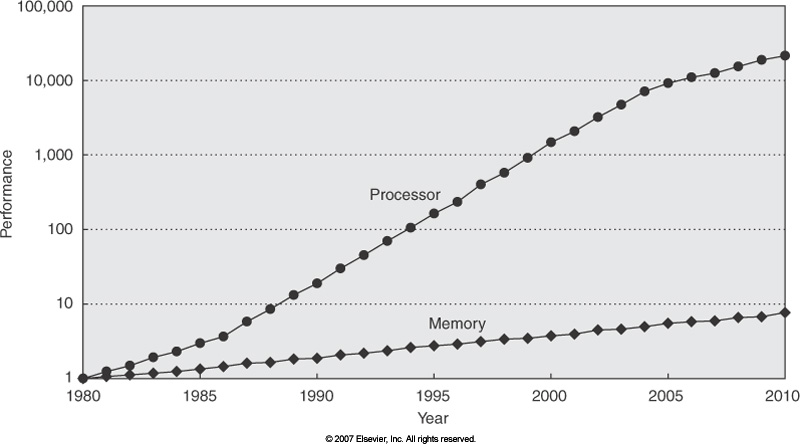
\includegraphics[scale=0.3]{./img/mem_gap}
	\caption{The memory gap}
	\label{img:mem_gap}
\end{figure}

The illusion will only partially hold, however, as the processor is
delayed for the entire main memory access time when the memory contents required
is not present in any of the caches. One technique
which has been introduced in order to face this problem is prefetching. Prefetching improves the utilization of the caches. This technique
attempts to improve the cache hit rate by predicting what memory
addresses the processor will want to access in the near future, and
issuing fetches from the main memory before the processor actually
needs the contents so that the data will reside in cache when the
processor does require it. This is usually accomplished by recording
memory access history and statistics, and using this to make educated
guesses about the future. 
{\bf (references, citations)}

\begin{figure}[H]
	\centering
	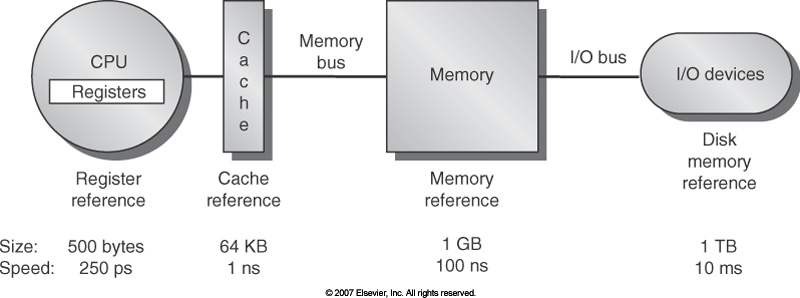
\includegraphics[scale=0.3]{./img/mem_hier}
	\caption{The memory hierarchy}
	\label{img:mem_hier}
\end{figure}

In this paper, we are going to investigate how different kinds of
prefetching strategies affects the efficiency of the prefetcher when
run on several different programs from the SPEC CPU2000 benchmark
suite.  {\bf (references, citations)}

\section{Solution}

% Evaluation criterion:
%- Language and use of figures
%- Clarity of the problem statement
%- Overall document structure
%- Depth of understanding for the field of computer architecture
%- Depth of understanding of the investigated problem

\section{Result}
\label{sec:result}

The speedup from when running the selected applications with the
different prefetchers is tabulated in \autoref{fig:initResults}.

\begin{figure}[ht]
  \centering
  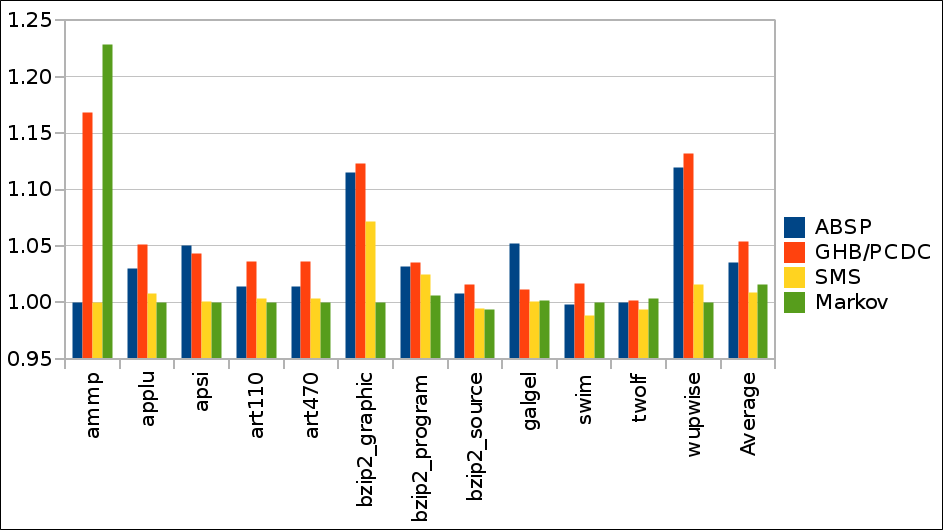
\includegraphics[scale=0.25]{figures/init_results.png}
  \caption{\label{fig:initResults} Speedup on the Y-axis plotted
    against program on the X-axis.}
\end{figure}

What other results? Should we include parameter search results? What
about results from experimenting with altering the prefetchers---does
that belong here or in the discussion section?XS

\subsection{Sequential Prefetcher Result}
\label{sec:sequentialPrefetcherResult}

\subsection{GHB Prefetcher Result}
\label{sec:ghbPrefetcherResult}

\subsection{Markov Prefetcher Result}
\label{sec:markovPrefetcherResult}

\subsection{Spatial Memory Streaming Prefetcher Result}
\label{sec:smsPrefetcherResult}


% Evaluation criterion:
%- Language and use of figures
%- Clarity of the problem statement
%- Overall document structure
%- Depth of understanding for the field of computer architecture
%- Depth of understanding of the investigated problem

\section{Discussion} % (fold)
\label{sec:discussion}

Can only be written when results are present.
Things to consider:

- How well do the different prefetchers perform on average?

- Are there any variance as to which programs they yield good speedup
on?

- How would combining them work?

- Considering how the time spent by our prefetching algorithms is not
taken into account, are our results at all accurate and usable?

- Anything else?

{\bf (references, citations)}

\section{Conclusion}

\begin{appendices}
\appendixpage

\section{MIPS Reference Data}\label{MIPS_SHEET}
%\includepdf[pages={1,2}]{MIPS_Green_Sheet.pdf}

\section{RTL schematics}
\label{RTL}
%\includepdf[pages={1}, angle=-90]{RTL.pdf}
\end{appendices}

\end{document}
